\documentclass[border=8pt]{standalone}
\usepackage[T1]{fontenc}
\usepackage{lmodern}
\usepackage{tikz}
\usetikzlibrary{arrows.meta, positioning, calc, fit, backgrounds}
\usepackage{pifont}

% ── Colour palette ──────────────────────────────────────────────
\definecolor{vulnRed}{HTML}{C0392B}
\definecolor{vulnRedBg}{HTML}{FADBD8}
\definecolor{fixGreen}{HTML}{27AE60}
\definecolor{fixGreenBg}{HTML}{D5F5E3}
\definecolor{altBlue}{HTML}{2980B9}
\definecolor{altBlueBg}{HTML}{D6EAF8}
\definecolor{boxGray}{HTML}{F2F3F4}
\definecolor{borderGray}{HTML}{BDC3C7}
\definecolor{textDark}{HTML}{2C3E50}
\definecolor{stampRed}{HTML}{E74C3C}

\begin{document}
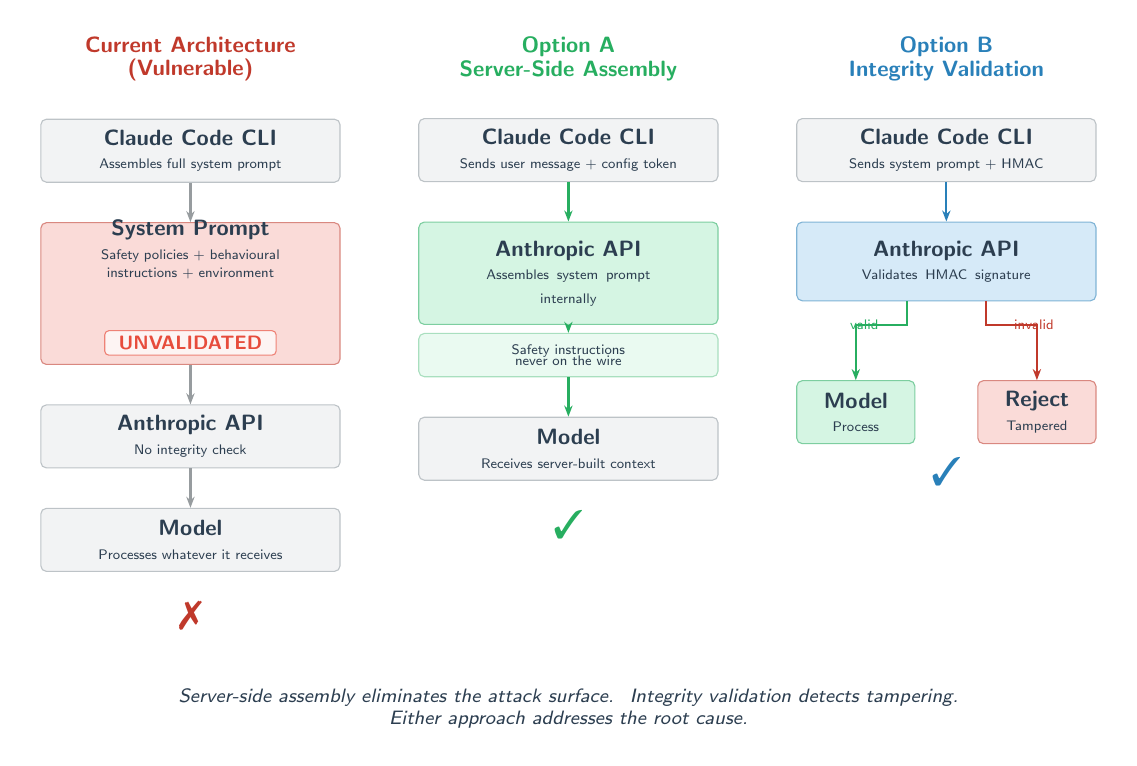
\begin{tikzpicture}[
    font=\sffamily\small,
    >={Stealth[length=4pt,width=3pt]},
    node distance=0.55cm,
    comp/.style={
        rectangle, rounded corners=2pt, draw=borderGray,
        fill=boxGray, minimum width=3.8cm, minimum height=0.8cm,
        align=center, text=textDark, font=\sffamily\footnotesize},
    vulnBox/.style={comp, fill=vulnRedBg, draw=vulnRed!60},
    greenBox/.style={comp, fill=fixGreenBg, draw=fixGreen!60},
    blueBox/.style={comp, fill=altBlueBg, draw=altBlue!60},
    colTitle/.style={font=\sffamily\footnotesize\bfseries, text=textDark, align=center},
    arr/.style={->, thick, color=borderGray!80!black},
    arrGreen/.style={->, thick, color=fixGreen},
    arrRed/.style={->, thick, color=vulnRed},
    arrBlue/.style={->, thick, color=altBlue},
    verdict/.style={font=\Large},
]

% Column spacing
\def\colsep{4.8cm}

% ── COLUMN 1 — Vulnerable ─────────────────────────────────────
\node[colTitle, text=vulnRed] (t1) at (0,0)
    {Current Architecture\\[-1pt]\footnotesize(Vulnerable)};

\node[comp, below=0.35cm of t1] (cli1)
    {\textbf{Claude Code CLI}\\[-1pt]
     {\tiny Assembles full system prompt}};

% System Prompt box — taller to fit stamp below text
\node[vulnBox, below=0.5cm of cli1, minimum height=1.8cm, text width=3.4cm] (sp1) {};
% Text at top of box
\node[font=\sffamily\footnotesize, text=textDark, align=center]
    at ($(sp1.north)+(0,-0.35)$)
    {\textbf{System Prompt}\\[-1pt]
     {\tiny Safety policies + behavioural}\\[-3pt]
     {\tiny instructions + environment}};
% Stamp badge at bottom of box
\node[font=\sffamily\scriptsize\bfseries, text=stampRed,
      inner sep=2pt, inner xsep=5pt,
      draw=stampRed!70, rounded corners=1.5pt,
      fill=white, fill opacity=0.7, text opacity=1]
    at ($(sp1.south)+(0,0.28)$) {UNVALIDATED};

\node[comp, below=0.5cm of sp1] (api1)
    {\textbf{Anthropic API}\\[-1pt]
     {\tiny No integrity check}};

\node[comp, below=0.5cm of api1] (mod1)
    {\textbf{Model}\\[-1pt]
     {\tiny Processes whatever it receives}};

\node[verdict, below=0.25cm of mod1, text=vulnRed] (x1)
    {\ding{55}};

\draw[arr] (cli1) -- (sp1);
\draw[arr] (sp1) -- (api1);
\draw[arr] (api1) -- (mod1);

% ── COLUMN 2 — Server-Side Assembly ───────────────────────────
\node[colTitle, text=fixGreen] (t2) at (\colsep,0)
    {Option A\\[-1pt]\footnotesize Server-Side Assembly};

\node[comp, below=0.35cm of t2] (cli2)
    {\textbf{Claude Code CLI}\\[-1pt]
     {\tiny Sends user message + config token}};

\node[greenBox, below=0.5cm of cli2, minimum height=1.3cm, text width=3.4cm] (api2)
    {\textbf{Anthropic API}\\[-1pt]
     {\tiny Assembles system prompt}\\[-1pt]
     {\tiny internally}};

\node[comp, below=0.1cm of api2, minimum height=0.55cm,
      fill=fixGreenBg!50, draw=fixGreen!40,
      font=\sffamily\tiny, text width=3.2cm] (note2)
    {Safety instructions\\[-2pt] never on the wire};

\node[comp, below=0.5cm of note2] (mod2)
    {\textbf{Model}\\[-1pt]
     {\tiny Receives server-built context}};

\node[verdict, below=0.25cm of mod2, text=fixGreen] (c2)
    {\ding{51}};

\draw[arrGreen] (cli2) -- (api2);
\draw[arrGreen] (api2) -- (note2);
\draw[arrGreen] (note2) -- (mod2);

% ── COLUMN 3 — Integrity Validation ──────────────────────────
\node[colTitle, text=altBlue] (t3) at (2*\colsep,0)
    {Option B\\[-1pt]\footnotesize Integrity Validation};

\node[comp, below=0.35cm of t3] (cli3)
    {\textbf{Claude Code CLI}\\[-1pt]
     {\tiny Sends system prompt + HMAC}};

\node[blueBox, below=0.5cm of cli3, minimum height=1.0cm, text width=3.4cm] (api3)
    {\textbf{Anthropic API}\\[-1pt]
     {\tiny Validates HMAC signature}};

% Branch targets — centered under column, compact spacing
\node[comp, minimum width=1.5cm,
      fill=fixGreenBg, draw=fixGreen!60,
      below=1.0cm of api3, xshift=-1.15cm] (mod3)
    {\textbf{Model}\\[-1pt]{\tiny Process}};

\node[comp, minimum width=1.5cm,
      fill=vulnRedBg, draw=vulnRed!60,
      below=1.0cm of api3, xshift=1.15cm] (rej3)
    {\textbf{Reject}\\[-1pt]{\tiny Tampered}};

% Branch arrows with labels
\draw[arrGreen] ($(api3.south)-(0.5,0)$)
    -- ++(0,-0.3)
    -| (mod3.north)
    node[pos=0.15, left=1pt, font=\sffamily\tiny, text=fixGreen]{valid};
\draw[arrRed] ($(api3.south)+(0.5,0)$)
    -- ++(0,-0.3)
    -| (rej3.north)
    node[pos=0.15, right=1pt, font=\sffamily\tiny, text=vulnRed]{invalid};

% Checkmark centered under column
\node[verdict, text=altBlue] (c3) at
    ($(mod3.south)!0.5!(rej3.south)+(0,-0.35)$) {\ding{51}};

\draw[arrBlue] (cli3) -- (api3);

% ── Bottom spanning caption ────────────────────────────────────
\path let \p1=(x1.south), \p2=(c2.south), \p3=(c3.south) in
    coordinate (lowestPt) at (\colsep, {min(\y1,min(\y2,\y3))});

\node[below=0.5cm of lowestPt, text width=13.5cm, align=center,
      font=\sffamily\scriptsize, text=textDark] (caption)
    {\emph{Server-side assembly eliminates the attack surface.\;
     Integrity validation detects tampering.\\
     Either approach addresses the root cause.}};

\end{tikzpicture}
\end{document}
